\documentclass{article}

\usepackage[a4paper,margin=1in]{geometry}
\usepackage{graphicx}
\usepackage{booktabs}
\newcommand{\tableinput}[1]{\csname @@input\endcsname #1 }
\usepackage{tabularx}
\usepackage{amsmath}
\usepackage{url}
\usepackage{caption}
\usepackage{float}
\captionsetup[figure]{name=Fig.,labelfont=bf,labelsep=space}

\graphicspath{{figures/}}

\title{Online Resource 1: Additional Reproducibility Details}
\author{\begin{tabular}{c}Cong Thanh Bui, Van Anh Nguyen, The Hung Nguyen, Anh Tu Nguyen,\\ Thi Quynh Le, Thi Linh Lai, and Trung Dung Nguyen\end{tabular}}
\date{}

\begin{document}
\maketitle

\noindent\textbf{Article title:} Budgeted Page-Level Preprocessing Selection for Vietnamese Administrative OCR: A Controlled Comparison of Learned, Retrieval-Based, and Static Shortlists

\noindent\textbf{Journal name:} International Journal on Document Analysis and Recognition

\noindent\textbf{Corresponding author:} Van Anh Nguyen, National Laboratory for Securing Information (NLSI), Ministry of National Defence, Hanoi, Vietnam. Email: \texttt{nguyenanhbh14@gmail.com}

\bigskip
\noindent\textbf{Caption:} Additional dataset summary, sampled-pool oracle improvement, offline OCR evaluation loop, preprocessing search-space table, surrogate feature groups, nested-CV surrogate model quality, nested GroupKFold protocol details and stepwise algorithm, policy-agnostic headroom controls, Vietnamese best-of-K curves, strict policy-matched and rank-only oracle-free selector results, SROIE intermediate-budget results omitted from the main manuscript, post hoc standalone-feature sensitivity, and contour-suppression schematic referenced from the main manuscript.

\section{Dataset Summary}

\begin{table}[h]
\centering
\caption{Dataset summary.}
\begin{tabularx}{\textwidth}{p{3.2cm} X X}
\toprule
Aspect & Vietnamese administrative documents & SROIE receipt images \\
\midrule
Dataset/domain & Vietnamese government administrative documents & SROIE receipt images \\
Source & Public Vietnamese Government document portal: \url{https://chinhphu.vn/he-thong-van-ban} & ICDAR 2019 SROIE benchmark \\
Images & 300 first-page images & 612 images after filename-level, exact-content and same-receipt filtering \\
Time span & 2015--2024, balanced by year & Not applicable \\
Reference text & Manually transcribed from images without consulting OCR; subsequent targeted checks; frozen v3 & Benchmark-provided full-text transcriptions; casefolded for primary CER \\
OCR recognizers & VietOCR, Tesseract, EasyOCR & Tesseract, EasyOCR \\
\bottomrule
\end{tabularx}
\end{table}

The final Vietnamese cohort preserves 30 first pages per year. An exact-content audit removed two duplicated selections and replaced them within their corresponding 2018 and 2024 strata before all reported Vietnamese experiments were recomputed; the public cohort manifest records final identifiers and image/reference SHA-256 hashes.

SROIE filtering first removed both members of five byte-identical pairs (626 to 616 receipts). A later screen of all 189,420 remaining image pairs produced 2,027 candidates. Targeted image review resolved two same-receipt pairs and 2,025 different-receipt comparisons: 49 direct pair reviews and 1,978 comparisons using image-verified transaction identifiers. This is not exhaustive duplicate-recall certification or a second independent human audit. Both members of the two confirmed pairs were excluded, leaving 612 pages and 30,600 candidate rows. All affected SROIE surrogate and nested selector/control training layers were rerun. New GroupKFold sizes are 123/123/122/122/122; 593 retained pages change numerical fold label relative to the 616-page cohort. Both metrics and Full/Drop share the new folds. Consequently, old/new differences include changed partitions, not an isolated duplicate-removal effect. Original outputs and exclusion/hash records remain available separately.

\section{Sampled-Pool Oracle Improvement}

\begin{table}[ht]
\centering
\caption{Sampled-pool oracle improvement over exact NoPre. Relative improvement is computed per page as $(\mathrm{NoPre}-\mathrm{SampOracle})/\mathrm{NoPre}$.}
\label{tab:oracle_improvement}
\small
\begin{tabular}{l l r r r}
\toprule
Setting & Recognizer & Pages improved & Mean rel. & Median rel. \\
\midrule
\tableinput{primary_tables/oracle_improvement.tex}
\bottomrule
\end{tabular}
\end{table}

\section{Offline OCR Evaluation Loop}

\noindent\textbf{Input:} Page images and references \(\mathcal{D}\); candidate pool \(\Theta\); recognizer set \(E\); optional contour transform \(C\).

\noindent\textbf{Output:} Collected data table with one row for each page \(i\) and preprocessing setting \(\theta_j\), containing page features, preprocessing settings, and observed CER values as regression targets.

\begin{enumerate}
    \item For each page \(x_i\), choose the page representation \(\tilde{x}_i\): \(x_i\) for raw experiments or \(C(x_i)\) for contour-suppressed experiments.
    \item Extract OCR-free page features \(f(\tilde{x}_i)\) once for that page representation.
    \item For each candidate \(\theta_j \in \Theta\), apply \(P_{\theta_j}\) to \(\tilde{x}_i\).
    \item For each recognizer \(e \in E\), run the initial shared-detection and backend-specific crop-processing pipeline and compute \(y_{i,j,e}\) by page-level CER against \(r_i\).
    \item Store \(z_{i,j}\), \(\theta_j\), page/fold identifiers, and CER targets \(y_{i,j,e}\).
\end{enumerate}

\section{Preprocessing Search Space}

\begin{table}[h]
\centering
\caption{Page-level preprocessing search space.}
\begin{tabularx}{\textwidth}{p{3.2cm} p{3.0cm} p{2.2cm} X}
\toprule
Parameter & Range & Off value & Role \\
\midrule
\texttt{gaussian\_ksize} & \{0, 3, 5, 7\} & 0 & denoising \\
\texttt{bilateral\_d} & \{0, \ldots, 9\} & 0 & edge-preserving denoising \\
\texttt{clahe\_clip} & [0, 4.0] & 0 & local contrast enhancement \\
\texttt{gamma} & [0.5, 1.5] & 1.0 & brightness correction \\
\texttt{sharpen} & [0, 2.0] & 0 & sharpening strength \\
\bottomrule
\end{tabularx}
\end{table}

A post hoc check with OpenCV 4.10 and the fixed bilateral-filter sigmas found that encoded positive diameters 1--3, 4--5, 6--7, and 8--9 gave identical outputs within each group; \texttt{bilateral\_d=0} is off. The original 50-candidate pool is retained despite this observed parameter redundancy.

A post hoc projection-profile diagnostic on all 300 raw Vietnamese pages gave median and maximum absolute skew estimates of $0.15^\circ$ and $1.40^\circ$. It searched $\pm5^\circ$ in $0.05^\circ$ steps on padded Otsu ink masks (width capped at 1,000 pixels), maximizing squared adjacent differences in horizontal projection. These estimator-dependent values do not establish deskew's effect on OCR, which was not tested. The stored Hough feature and fitted models were unchanged. Script, configuration, per-page estimates, score curves and hashes accompany the public release.

\section{Surrogate Feature Groups}

\begin{table}[h]
\centering
\caption{Surrogate feature groups.}
\begin{tabularx}{\textwidth}{p{3.0cm} p{6.2cm} X}
\toprule
Feature group & Features & Purpose \\
\midrule
Base image features & blur, contrast, brightness, \texttt{noise}, edge density, entropy, dynamic range & blur is Laplacian variance; \texttt{noise} is Laplacian standard deviation, its square root, not an independent noise estimate \\
Document-aware features & text density, skew angle, connected-component count, aspect ratio, estimated line count & capture page structure not represented by intensity statistics alone \\
Preprocessing parameters & \texttt{gaussian\_ksize}, \texttt{bilateral\_d}, \texttt{clahe\_clip}, \texttt{gamma}, \texttt{sharpen} & describe the candidate preprocessing setting being scored \\
Interaction terms & blur $\times$ \texttt{gaussian\_ksize}, contrast $\times$ \texttt{clahe\_clip}, brightness $\times$ \texttt{gamma}, noise $\times$ \texttt{bilateral\_d}, entropy $\times$ \texttt{sharpen} & encode predefined relationships between page properties and preprocessing controls \\
\bottomrule
\end{tabularx}
\end{table}

\section{Nested-CV Surrogate Model Quality}

\begin{table}[h]
\centering
\caption{Nested-CV surrogate model quality. Spearman values are reported as mean $\pm$ standard deviation across outer folds. The final refit model is selected and fitted on all available pages; reported metrics are out-of-fold nested-CV results and do not use this final model.}
\small
\resizebox{\textwidth}{!}{%
\begin{tabular}{l l l r r r r}
\toprule
Setting & Recognizer & Final refit model & MAE & $R^2$ & Global Spearman & Per-image Spearman \\
\midrule
\tableinput{primary_tables/model_quality.tex}
\bottomrule
\end{tabular}%
}
\end{table}

\section{Nested GroupKFold Protocol}

\begin{table}[h]
\centering
\caption{Nested GroupKFold evaluation protocol.}
\begin{tabularx}{\textwidth}{p{3.1cm} p{4.2cm} X}
\toprule
Component & Setting & Purpose \\
\midrule
Outer evaluation split & 5-fold GroupKFold grouped by page image & prevents rows from the same page appearing in both training and test data \\
Outer test unit & held-out pages, with all 50 candidates kept together & produces out-of-fold page-level evaluation \\
Inner model selection & 5-fold GroupKFold on each outer training split & selects the surrogate model family by validation MAE without using outer test pages \\
Reported aggregation & held-out page-level results combined across the five outer folds & provides one out-of-fold result per page for CER summaries and statistical tests \\
Final refit & model family selected and refit on all available pages & final model is not used to compute reported cross-validation metrics \\
\bottomrule
\end{tabularx}
\end{table}

\section{Nested GroupKFold Evaluation Algorithm}

\noindent\textbf{Input:} Collected data table; candidate pool \(\Theta\); recognizer \(e\); \(K\) values \(\{3,5,10,15\}\); model-family set \(\mathcal{H}\).

\noindent\textbf{Output:} Out-of-fold page-level Surrogate K, Random K, FixedTopK, NN-K, FixedBest, NoPre, and sampled-oracle results.

\begin{enumerate}
    \item Split pages into five outer GroupKFold folds, keeping all 50 candidate rows from the same page in the same fold.
    \item For each outer fold, select \(h_e \in \mathcal{H}\) by inner GroupKFold validation MAE on the outer-training pages.
    \item Refit the selected model on all outer-training rows and score all \(\theta_j\in\Theta\) for each held-out page.
    \item Compute Surrogate K, Random K, FixedTopK, NN-K, FixedBest, NoPre, and sampled-oracle references using the definitions in the main manuscript.
    \item Pool held-out page-level results across the five outer folds.
    \item Compute mean CER, bootstrap confidence intervals, and two-sided Wilcoxon signed-rank tests with SciPy \texttt{zero\_method=wilcox} (zero paired differences excluded from signed ranks).
    \item Apply Holm correction within each policy-contrast/evaluation-block family; retain both raw and adjusted p-values.
\end{enumerate}

The inner loop selects the surrogate model family by candidate-level validation MAE. This preserves test-fold separation but is only indirectly aligned with the downstream within-page ranking and best-of-K objective.

\section{Policy-Agnostic Headroom Controls}

For each held-out page and budget, the main manuscript defines FixedTopK-to-oracle headroom as \(H=F-O\). The coupled outcomes \(F-P\), for policy \(P\), share \(F\) with \(H\) and satisfy \(F-P\leq F-O\). We therefore recomputed the correlation for Surrogate, Random, and NN-K and added direct policy-to-policy controls that do not contain FixedTopK. At every budget, all eight dataset/setting/recognizer configurations have significantly positive coupled correlations for all three policies after Holm correction within each policy's 32-correlation family. Table~\ref{tab:headroom_control_breakdown} gives the per-budget breakdown of the additional controls.

\begin{table}[h]
\centering
\caption{Per-budget headroom-control breakdown. Random $r>$ Surrogate $r$ compares the two coupled correlations. The remaining columns count significantly positive Spearman correlations after Holm correction within each direct outcome's 32-correlation family. Each budget contains eight dataset/setting/recognizer configurations.}
\label{tab:headroom_control_breakdown}
\small
\resizebox{\textwidth}{!}{%
\begin{tabular}{r r r r r r}
\toprule
\(K\) & Coupled positive, each policy & Random \(r>\) Surrogate \(r\) & Random $-$ Surrogate & Random $-$ NN-K & NN-K $-$ Surrogate \\
\midrule
\tableinput{primary_tables/headroom_budget.tex}
\bottomrule
\end{tabular}%
}
\end{table}

Across budgets, coupled correlations remain positive and significant in 32/32 configurations for each policy; Random has a larger correlation than Surrogate in 30/32. The direct Random-minus-Surrogate correlation ranges from $-0.502$ to $-0.057$, is negative in 32/32 and significantly negative in 28/32 after Holm correction. These controls support a policy-agnostic, retrospective interpretation of headroom.

\clearpage
\section{Vietnamese Best-of-K Curves}

\begin{figure}[H]
\centering
\textbf{(a) Raw}\par\smallskip
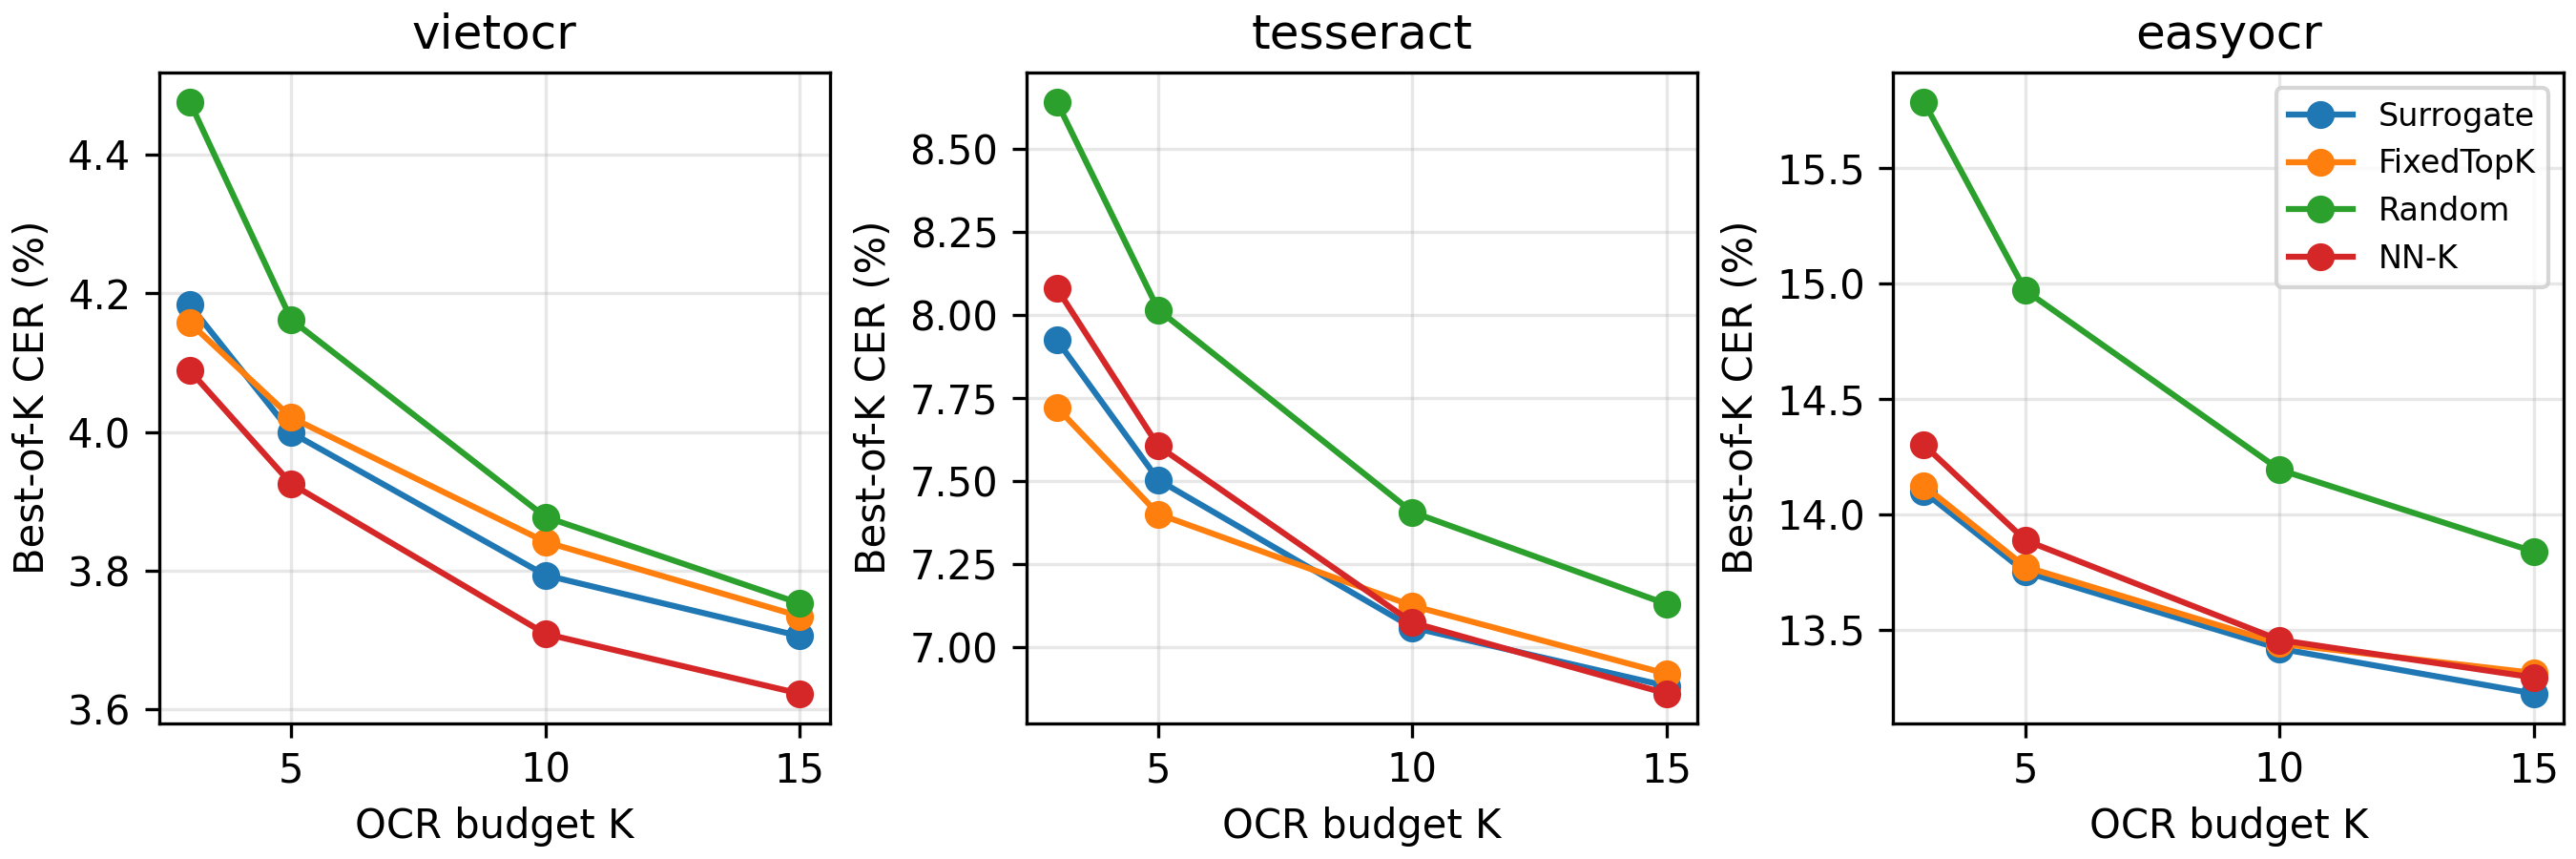
\includegraphics[width=\textwidth]{raw_pareto_multiengine.png}
\par\medskip
\textbf{(b) Contour}\par\smallskip
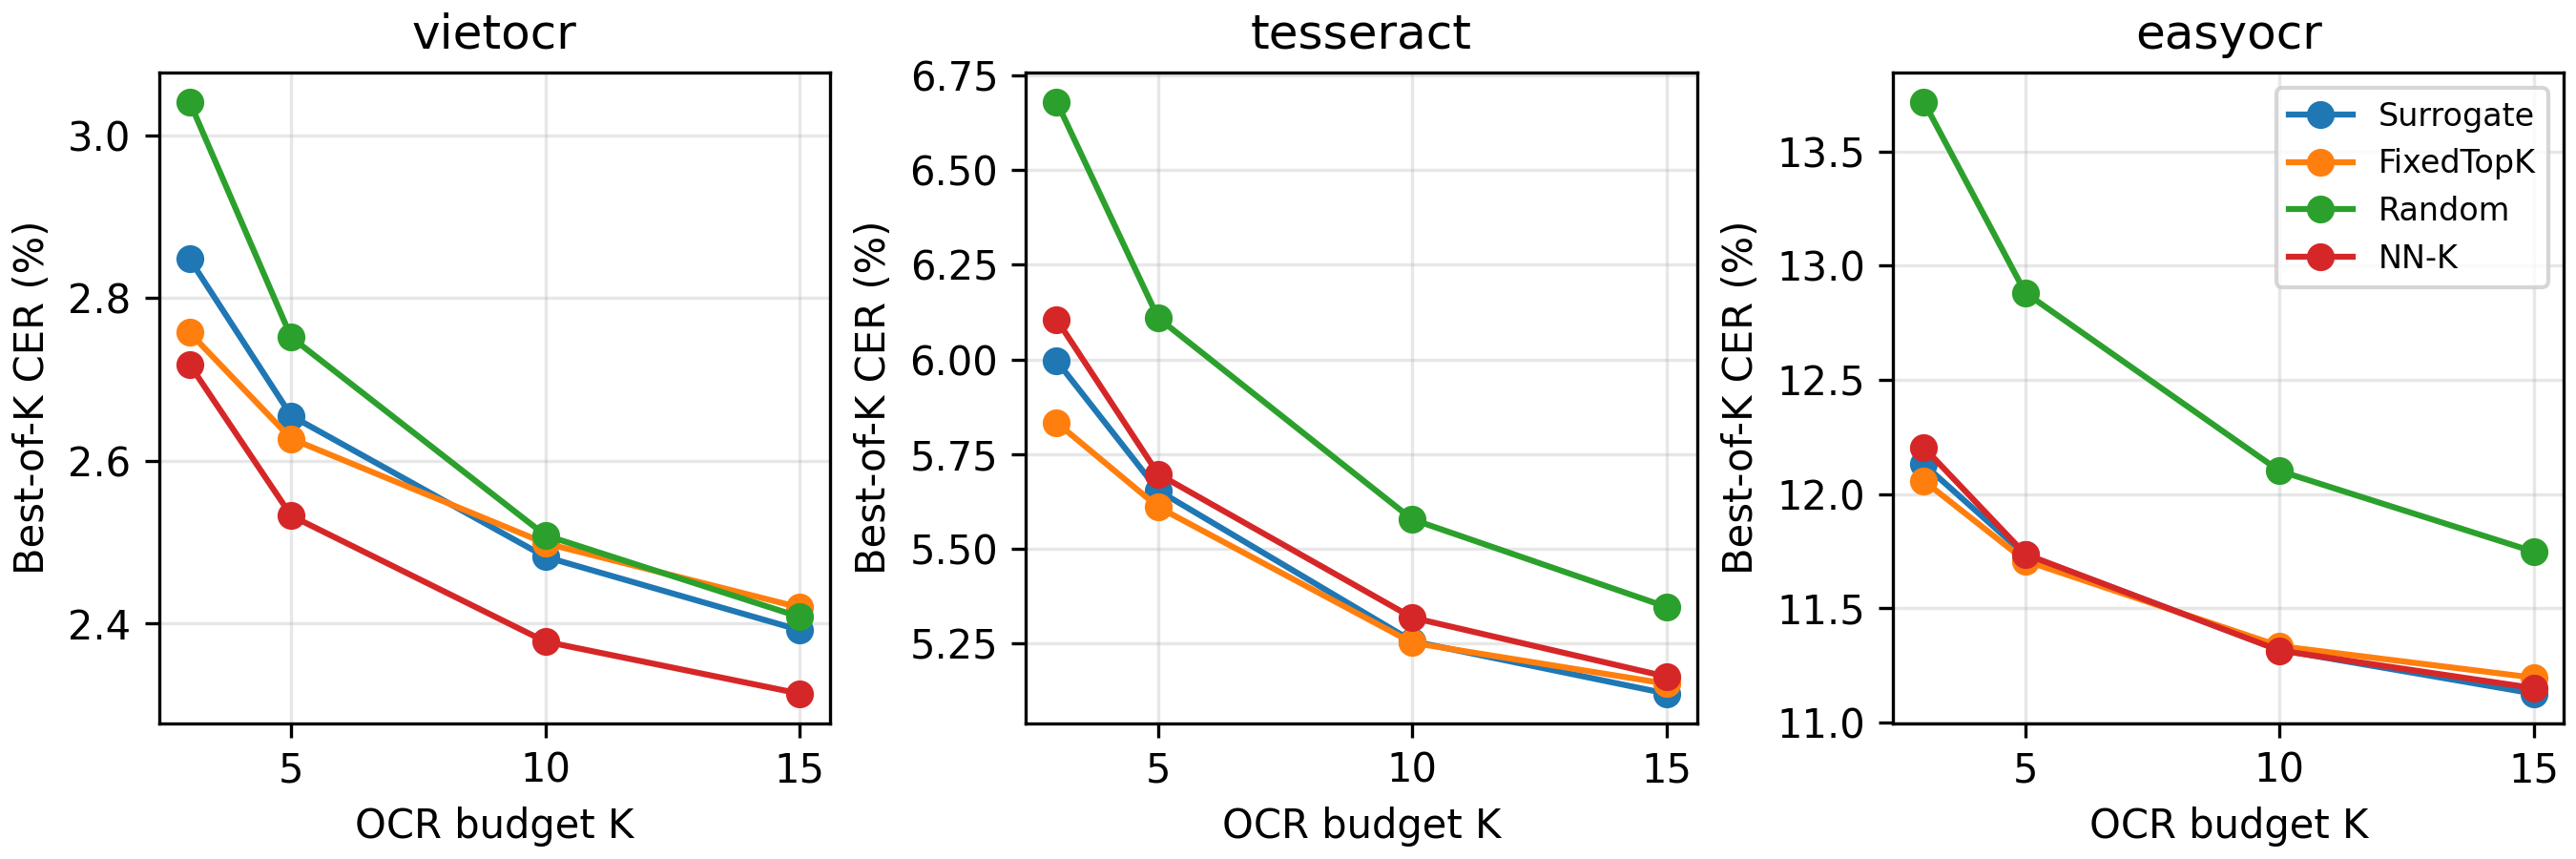
\includegraphics[width=\textwidth]{contour_pareto_multiengine.png}
\caption{Mean best-of-K CER for Surrogate, FixedTopK, Random, and NN-K on Vietnamese administrative documents: (a) raw pages and (b) contour-suppressed pages. Surrogate/Random values match main-manuscript Table~1, and FixedTopK values at $K=3,15$ match Table~2; all plotted values are available in the public tables. Each recognizer panel uses its own y-axis scale}
\end{figure}

\section{Multiplicity-Adjusted Best-of-K Policy Comparisons}

For best-of-K inference, each policy contrast within one evaluation block is a Holm family: 12 recognizer-budget tests in each Vietnamese block and eight tests on SROIE. Table~\ref{tab:policy_holm_counts} reports direction-specific counts before and after correction. ``A lower'' means lower mean CER for the first policy named in the contrast; ``B lower'' means lower mean CER for the second.

\begin{table}[H]
\centering
\caption{Direction-specific significant comparison counts. Each cell is unadjusted/Holm-adjusted; Holm correction is within the block and contrast shown.}
\label{tab:policy_holm_counts}
\small
\resizebox{\textwidth}{!}{%
\begin{tabular}{l l r r}
\toprule
Block & Contrast (A vs B) & A lower & B lower \\
\midrule
\tableinput{primary_tables/policy_counts.tex}
\bottomrule
\end{tabular}%
}
\end{table}

At $K=15$, EasyOCR has 215/300 zero Surrogate--FixedTopK differences in raw and 216/300 in contour. Table~\ref{tab:vn_zero_sensitivity} reports a post hoc zero-handling check using separate 12-test families for each block and convention. The specified \texttt{wilcox} analysis remains primary; its apparent advantage in contour, and the advantages found under other conventions in raw, are sensitive to zero handling. The adverse contour VietOCR $K=3$ result remains significant under all three checked conventions.

\begin{table}[h]
\centering\small
\caption{EasyOCR $K=15$ zero-handling sensitivity. Differences are Surrogate minus FixedTopK (pp). Holm correction uses 12 tests per block and convention.}
\label{tab:vn_zero_sensitivity}
\begin{tabular}{l l r r r}
\toprule Block & Zero method & Zero pages & Diff & Holm $p$ \\
\midrule\tableinput{primary_tables/zero_sensitivity.tex}\bottomrule
\end{tabular}\end{table}

\section{SROIE Letter-Case Metric Transition and Case-Sensitive Sensitivity}
\label{sec:sroie_casefold}

The primary SROIE results in this revision use casefolded CER. The original analysis was case-sensitive, and the metric decision was changed after initial results and the casefold best-of-K sensitivity were available. Inspection of letter-case fidelity motivated the change; it was not prespecified before those results. Rotman et al.\ \cite{rotman2022masking} likewise use case-insensitive edit-distance evaluation for SROIE because its annotations do not preserve letter case, although their evaluation is not identical to ours. Baek et al.\ \cite{baek2019wrong} report case-related annotation inconsistencies in other scene-text benchmarks; that observation does not establish annotation errors in SROIE.

Both predictions and references receive the same NFC and whitespace normalization, with Unicode casefold additionally applied for SROIE. Accents and punctuation are retained. Vietnamese evaluation remains case-sensitive on corrected v3 references. Surrogate targets, train-only static rankings, NN-K transfer choices and all nested SROIE selector/control training targets were updated consistently. Selector text-composition and agreement features are computed from the original OCR strings, not casefolded strings.

Tables~\ref{tab:sroie_casefold_counts} and~\ref{tab:sroie_casefold_nn} compare both metrics on the same corrected 612 receipts, 50 candidates and new outer folds. Earlier 616-page results remain historical, not the numerical source of these tables. Surrogate and NN-K outperform Random and FixedTopK in 8/8 comparisons under both metrics. Surrogate is significantly better than NN-K for Tesseract $K=3,5,10$ under both metrics. NN-K's EasyOCR $K=5$ advantage is significant under both metrics; its $K=3$ advantage is significant under casefolding ($p_H=0.0336$) but not case-sensitive CER ($p_H=0.0778$). Crossing a significance threshold is not a formal metric-by-policy interaction test, nor does nonsignificance establish equivalence.

Each metric/contrast has a separate eight-test Holm family using two-sided Wilcoxon and the \texttt{wilcox} zero convention. Mean-difference CIs are per-comparison 95\% paired percentile intervals, with 10,000 resamples and recorded seeds, not multiplicity-adjusted. Nonzero rounded-zero endpoints retain their signs. Significance statements use Wilcoxon--Holm, not CI zero exclusion; for example, the Tesseract $K=10$ NN-K--Surrogate mean-difference intervals contain zero under both metrics despite significant signed-rank tests. Historical BCa and multiple-seed diagnostics on 616 receipts remain archived but were not repeated for these 612-page intervals and do not validate their coverage.

\begin{table}[H]
\centering\small
\caption{Matched 612-receipt best-of-$K$ sensitivity: Holm-significant lower-CER counts. Each metric/contrast has a separate eight-test family; A/B identifies the lower-CER policy.}
\label{tab:sroie_casefold_counts}
\begin{tabular}{lcc}\toprule
Contrast (A vs B) & Case-sensitive A/B & Casefold A/B \\\midrule
Surrogate vs Random & 8/0 & 8/0 \\
Surrogate vs FixedTopK & 8/0 & 8/0 \\
NN-K vs Random & 8/0 & 8/0 \\
NN-K vs FixedTopK & 8/0 & 8/0 \\
NN-K vs Surrogate & 1/3 & 2/3 \\
\bottomrule\end{tabular}\end{table}

\begin{table}[H]
\centering\small
\caption{NN-K minus Surrogate on the same 612 receipts and folds (pp). CS: case-sensitive sensitivity; CF: primary casefold. CIs are per-comparison 95\% paired percentile intervals, not multiplicity-adjusted; $p_H$ uses each metric\textquotesingle s eight-test family. Nonzero rounded-zero endpoints retain their signs. Significance follows Wilcoxon--Holm, not mean-CI zero exclusion.}
\label{tab:sroie_casefold_nn}
\resizebox{\textwidth}{!}{%
\begin{tabular}{lr r r r r r r}\toprule
Engine & $K$ & CS $\Delta$ & CS 95\% CI & CS $p_H$ & CF $\Delta$ & CF 95\% CI & CF $p_H$ \\\midrule
Tesseract & 3 & +0.53 & [+0.21, +0.86] & 0.00164 & +0.61 & [+0.28, +0.93] & 0.000261 \\
Tesseract & 5 & +0.34 & [+0.09, +0.59] & 0.00164 & +0.38 & [+0.14, +0.62] & 0.00254 \\
Tesseract & 10 & +0.16 & [-0.04, +0.35] & 0.00646 & +0.19 & [-0.01, +0.40] & 0.0343 \\
Tesseract & 15 & +0.03 & [-0.12, +0.18] & 0.151 & +0.09 & [-0.07, +0.26] & 0.125 \\
EasyOCR & 3 & -0.16 & [-0.27, -0.05] & 0.0778 & -0.16 & [-0.28, -0.03] & 0.0336 \\
EasyOCR & 5 & -0.13 & [-0.22, -0.05] & 0.0372 & -0.13 & [-0.23, -0.04] & 0.0191 \\
EasyOCR & 10 & -0.02 & [-0.08, +0.04] & 1.00 & -0.03 & [-0.11, +0.04] & 0.866 \\
EasyOCR & 15 & +0.03 & [-0.03, +0.08] & 1.00 & -0.01 & [-0.07, +0.05] & 0.798 \\
\bottomrule\end{tabular}}\end{table}


This cross-metric sensitivity directly compares best-of-K outputs only. Current casefold one-output selector results are reported below; historical case-sensitive selector artifacts are retained separately, but no formal paired cross-metric selector sensitivity is claimed.

\section{Policy-Matched Oracle-Free Selector Comparisons}

We compared complete one-output policies using strictly nested Surrogate, NN-K and FixedTopK top-3 selectors. The 16 full-feature comparisons form one Holm family. Surrogate is significantly better than NN-K on raw Tesseract and SROIE Tesseract, and better than FixedTopK on SROIE Tesseract. It is significantly worse than FixedTopK on contour VietOCR. The other 12 rows are not significant. Differences are Surrogate minus comparator in pp.

The 95\% bootstrap intervals in this and the rank-only table are pointwise intervals for the paired mean CER difference, not Holm-adjusted simultaneous intervals. Statistical-significance claims use the Holm-adjusted Wilcoxon p-values; the signed-rank test does not directly test a null hypothesis about the mean difference.

\begin{table}[h]
\centering
\caption{Strict policy-matched selector comparison. Holm p-values are adjusted across all 16 rows. CIs are per-comparison 95\% intervals, not multiplicity-adjusted. Nonzero bounds retain their signs when rounded: +0.00 or $-0.00$ does not mean exactly zero. Significance follows Holm-adjusted Wilcoxon tests, not CI zero exclusion.}
\label{tab:strict_policy_selector}
\scriptsize
\resizebox{\textwidth}{!}{%
\begin{tabular}{l l l r r r r r}
\toprule
Setting & Recognizer & Comparator & Surrogate & Comparator CER & Diff & 95\% CI & Holm $p$ \\
\midrule
\tableinput{primary_tables/full_policy.tex}
\bottomrule
\end{tabular}%
}
\end{table}

\section{Rank-Only Selector Sensitivity Analysis}

The main Surrogate selector uses continuous predictions and margins, whereas NN-K and FixedTopK provide an order. Replacing these prediction-related features by ranks preserves the exact surrogate top-3 candidates and OCR outputs before refitting the nested selector. CER changes by $-0.059$ to $+0.035$ pp relative to full features. The separate 16-test sensitivity family has three significant advantages (NN-K on raw/SROIE Tesseract, FixedTopK on SROIE Tesseract) and no significant disadvantages. This does not isolate shortlist quality because the selector is refit and retains OCR-output features.

\begin{table}[H]
\centering
\caption{Rank-only Surrogate selector sensitivity. Holm p-values are adjusted across all 16 rows in this separate sensitivity family. CIs are per-comparison 95\% intervals, not multiplicity-adjusted; signs of nonzero rounded endpoints are retained. Significance follows Holm-adjusted Wilcoxon tests.}
\label{tab:feature_matched_selector}
\scriptsize
\resizebox{\textwidth}{!}{%
\begin{tabular}{l l l r r r r r}
\toprule
Setting & Recognizer & Comparator & Rank-only Surr. & Comparator CER & Diff & 95\% CI & Holm $p$ \\
\midrule
\tableinput{primary_tables/rank_only_policy.tex}
\bottomrule
\end{tabular}%
}
\end{table}

\noindent\begin{minipage}{\textwidth}
\section{SROIE Intermediate-Budget Results}

\begin{table}[H]
\centering
\caption{SROIE receipt-setting intermediate-budget CER results. Values are percentages. These rows complement the main-manuscript SROIE table, which reports $K=3$ and $K=15$.}
\small
\resizebox{\textwidth}{!}{%
\begin{tabular}{l r r r r r}
\toprule
Recognizer & $K$ & Surrogate K & NN-K & FixedTopK & Random K \\
\midrule
\tableinput{primary_tables/sroie_intermediate.tex}
\bottomrule
\end{tabular}%
}
\end{table}
\end{minipage}
\par

\section{Post Hoc Standalone-Feature Sensitivity}
\label{sec:noise_feature_sensitivity}

The legacy \texttt{orig\_noise} column is the standard deviation of the Laplacian response, the square root of \texttt{orig\_blur}, rather than an independent noise estimate. After the primary results were available, a supplementary best-of-$K$ protocol was fixed before its fits: rerun the original input (Full: 22 surrogate and 12 NN-K columns) and remove only this standalone column (Drop: 21 and 11 columns). The interaction \texttt{inter\_noise\_bilateral\_d} was retained unchanged and means $\sqrt{\text{Laplacian variance}}\times\texttt{bilateral\_d}$. Both conditions used the same frozen references, CER rules, five page-group folds, candidate order, model definitions and seed 42. Nested surrogate selection and NN-K were rerun; strict one-output selectors were not. The primary 22/12-column results were retained regardless of this supplementary outcome. Removal can change model-family selection, stochastic column subsampling and NN distance weighting; this is not an isolated measurement of information content.

The original Vietnamese Full reruns reproduced primary per-page CER and model-family selections. For the corrected SROIE cohort, A and primary analyses reuse the identical verified Full outputs and new folds; Drop was fitted on that same cohort. Full reproduces all 160 primary policy-comparison rows. Direct Drop-minus-Full comparisons for Surrogate and NN-K used six separate policy-by-block Holm families (12 tests per Vietnamese block and eight for SROIE). The five existing policy contrasts were also recomputed under each condition using their original 15 block-by-contrast families. Tests were paired, two-sided Wilcoxon with \texttt{zero\_method=wilcox}. Conditional paired-page percentile 95\% CIs used 10,000 resamples with fixed recorded seeds; they are not multiplicity-adjusted and do not include refit, seed or split variability.

Table~\ref{tab:noise_direct_ranges} summarizes mean CER changes. None of the 64 direct Drop-minus-Full tests survives Holm correction. This does not establish equivalence or absence of a feature-removal effect; full-precision differences and unadjusted mean-difference CIs are released.

Seven of the 160 policy significance classifications changed (Table~\ref{tab:noise_changed_conclusions}), without reversing the mean-difference signs of those seven rows. Six Vietnamese comparisons lost significance, including both the contour EasyOCR $K=15$ Surrogate advantage and the contour VietOCR $K=3$ Surrogate disadvantage relative to FixedTopK. One SROIE comparison gained significance: Surrogate over NN-K for Tesseract $K=15$. Five other, nonsignificant Vietnamese mean contrasts reversed sign; all ten associated adjusted p-values equal 1. In both conditions, Surrogate and NN-K remained better than Random after Holm in all 24 Vietnamese and eight SROIE comparisons, and both remained better than FixedTopK in all eight SROIE comparisons. Secondary policy distinctions are nevertheless sensitive to the feature configuration; neither non-significance nor an unchanged classification establishes equivalence. A change in significance is not a formal test of the difference between contrasts. These best-of-$K$ results do not establish strict-selector robustness. Full-precision paired values, all 384 comparisons, the original design protocol, corrected-cohort provenance and arithmetic replay are included in the public supplement.

\begin{table}[htbp]
\centering\small
\caption{Standalone Laplacian-standard-deviation removal: range of Drop-minus-Full mean best-of-$K$ CER differences across engines and budgets (pp). Negative is lower CER after removal. The final column counts Holm-significant lower/higher results in each separate direct-comparison family. All 64 comparisons, including CIs, are released.}
\label{tab:noise_direct_ranges}
\begin{tabular}{llrrrr}\toprule
Setting & Policy & Minimum & Maximum & Tests & Lower/Higher \\\midrule
VN contour & NN-K & -0.03 & +0.02 & 12 & 0/0 \\
VN contour & Surrogate & -0.04 & +0.04 & 12 & 0/0 \\
VN raw & NN-K & -0.05 & +0.02 & 12 & 0/0 \\
VN raw & Surrogate & -0.06 & +0.04 & 12 & 0/0 \\
SROIE & NN-K & -0.06 & +0.07 & 8 & 0/0 \\
SROIE & Surrogate & -0.05 & +0.34 & 8 & 0/0 \\
\bottomrule\end{tabular}\end{table}

\begin{table}[htbp]
\centering\small
\caption{All 7 policy comparisons whose Holm-adjusted significance classification changes after removing only the standalone column. Differences are first policy minus second (pp); negative favors the first. $p_H$ uses the same prespecified block/contrast family in each condition (12 tests for each Vietnamese block, eight for SROIE). These threshold crossings are not formal tests of a difference between contrasts. Full-precision results for all 160 comparisons per condition are released.}
\label{tab:noise_changed_conclusions}
\resizebox{\textwidth}{!}{%
\begin{tabular}{lll l rrrr}\toprule
Setting & Engine & $K$ & Contrast & Full $\Delta$ & Drop $\Delta$ & Full $p_H$ & Drop $p_H$ \\\midrule
VN contour & EasyOCR & 15 & Surr.--FixedTopK & -0.07 & -0.07 & 0.0384 & 0.104 \\
VN contour & VietOCR & 3 & Surr.--FixedTopK & +0.09 & +0.09 & 0.0361 & 0.181 \\
VN contour & VietOCR & 10 & NN-K--FixedTopK & -0.12 & -0.12 & 0.0445 & 0.0507 \\
VN contour & VietOCR & 10 & NN-K--Surr. & -0.10 & -0.09 & 0.0371 & 0.138 \\
VN contour & VietOCR & 15 & NN-K--FixedTopK & -0.11 & -0.10 & 0.0189 & 0.0507 \\
VN raw & VietOCR & 10 & NN-K--FixedTopK & -0.13 & -0.13 & 0.0355 & 0.0656 \\
SROIE & Tesseract & 15 & NN-K--Surr. & +0.09 & +0.15 & 0.125 & 0.0306 \\
\bottomrule\end{tabular}}
\end{table}


\section{Contour Suppression: Schematic and Threshold Check}

The exploratory threshold check used VietOCR on the first three lexicographically sorted available PNG filenames from each of the ten Vietnamese year folders (30 pages total). Its saved report is dated 23 August 2026, before the later reference-NFC correction. It was not rerun on the final references or with Tesseract and EasyOCR.

Table~\ref{tab:contour_threshold_check} summarizes one-at-a-time threshold changes. The lower aspect-ratio bound remained fixed at 1.0 and was not tested. These are descriptive changes in sample mean CER, not per-page maxima or significance tests; they do not establish robustness on the final references.

\begin{table}[h]
\centering
\caption{Historical contour-threshold check on 30 pages with VietOCR. Default mean CER was 2.72\%. Each threshold was varied separately, with the others fixed at their defaults (area 500 square pixels, upper aspect ratio 5, width 80 pixels, height 30 pixels). Changes are relative to that default and expressed in percentage points.}
\label{tab:contour_threshold_check}
\small
\begin{tabular}{l l r}
\toprule
Threshold & Tested values & Max $|\Delta\mathrm{mean\ CER}|$ (pp) \\
\midrule
Area (px$^2$) & 500, 1000, 1500, 2000, 3000 & 0.56 \\
Upper aspect ratio & 3, 4, 5, 6, 8 & 0.06 \\
Minimum width (pixels) & 50, 60, 80, 100, 120 & 0.25 \\
Minimum height (pixels) & 15, 20, 30, 40, 50 & 0.29 \\
\bottomrule
\end{tabular}
\end{table}

\begin{figure}[h]
\centering
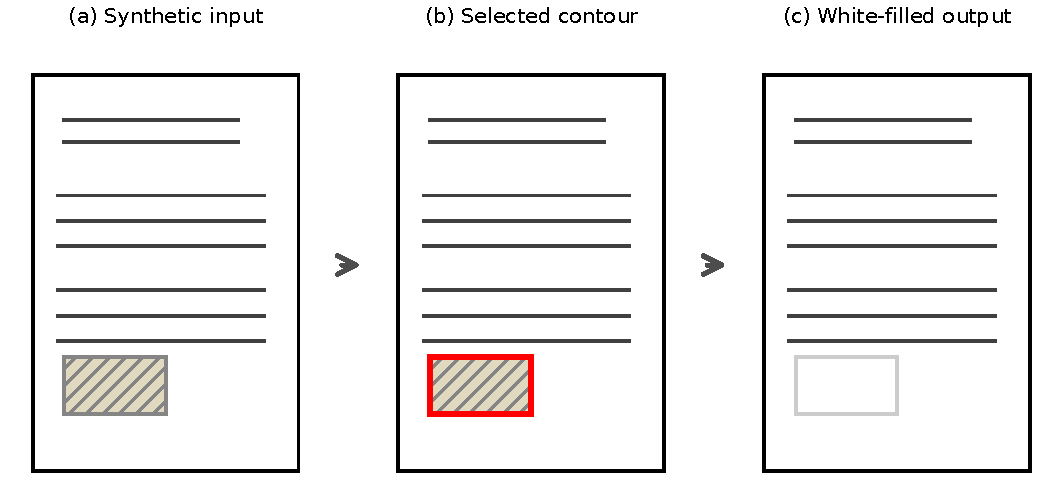
\includegraphics[width=0.75\linewidth]{contour_suppression_ijdar.pdf}
\caption{Synthetic illustration of contour suppression. A stamp-like rectangular artifact is identified and white-filled before OCR. The figure is schematic and does not reproduce a real source document}
\end{figure}

\bibliographystyle{plain}
\bibliography{reference}

\end{document}
